\documentclass[10pt, UKenglish]{beamer}
\usepackage{babel}
\usepackage[utf8]{inputenc}  
\usepackage{geometry}
\usepackage[customcolors]{hf-tikz}
\usepackage[T1]{fontenc}   
\usepackage{tcolorbox}
\usepackage{siunitx}
\usepackage{graphicx}
\usepackage{hyperref}
\usepackage{bookmark}
\usepackage{marvosym}
\usepackage{tikz}
\usepackage{tikz-qtree}
\usepackage{cancel}
\usepackage{todonotes}
\useoutertheme[subsection=false]{smoothbars}
\DeclareSIUnit[number-unit-product = {}]{\inchQ}{\textquotedbl}
\usepackage{amsmath,bm}
\DeclareSIUnit[number-unit-product = {\thinspace}]{\inch}{in}
\usetheme[menuwidth={0.3\paperwidth}]{erlangen}
\usepackage{multicol}
\usepackage{charter}
\setbeamercovered{transparent=20}
\setbeamertemplate{navigation symbols}{}
\sisetup{separate-uncertainty = true}
\usepackage[version=4]{mhchem}
\usepackage{tikz}
\usepackage{hepnames}
\usepackage{soul}
\usepackage{color}
\usepackage{thesis_defs}
\usepackage{subcaption}
\captionsetup[subfigure]{labelformat=empty}
\usepackage{xcolor}


\usepackage[backend=biber]{biblatex}
\bibliography{bibliography.bib}

\graphicspath{%
  {./feynman_diagrams/}%
  {./figures_theory/}%
  {./figures_simple/}%
  {./figures_misc/}%
  {./app1/}%
  {./app2/}%
  {./app3/}%
}


\definecolor{color1}{RGB}{33,217,217}
\definecolor{color2}{RGB}{7,61,111}

\newcommand{\lr}{\mathcal{lr}}


\newcounter{totavalue}
\newcounter{parvalue}

\def\aux{1}
\def\radius{9pt}
\def\step{4pt}
\usepackage[absolute,overlay]{textpos}


\newcommand\circcounter{%
\ifnum\inserttotalframenumber<2\relax
\else
  \setcounter{totavalue}{\inserttotalframenumber}
  \setcounter{parvalue}{\insertframenumber}
  \ifnum\inserttotalframenumber>45\relax
    \renewcommand\step{0pt}
  \fi%
  \pgfmathsetmacro{\aux}{360/27}
  \begin{tikzpicture}[remember picture,overlay, rotate=90+\aux]
  \foreach \i in {0,1,...,27}
    \fill[logo_blue] 
      (0,0) -- (-\i*\aux:\radius) arc  (-\i*\aux:-(\i+1)*\aux+\step:\radius) -- cycle;
  \foreach \i in {1,...,\insertframenumber}
    \fill[logo_grey] 
      (0,0) -- (-\i*\aux:\radius) arc  (-\i*\aux:-(\i+1)*\aux+\step:\radius) -- cycle;
  \fill[white] circle (\radius/1.3);
  \node at (0,0) {\small\insertframenumber}; 
  \end{tikzpicture}%
\fi%
}


\usepackage{eso-pic,picture}
\hypersetup{
    colorlinks=true,
    linkcolor=blue,
    filecolor=magenta,      
    urlcolor=cyan,
    pdftitle={Overleaf Example},
    pdfpagemode=FullScreen,
}




\begin{document} 

\title[tH(tautau) Review and plans]{tH($\tau\tau$) Review and plan}
\subtitle{\today}
\author{Christian Kirfel\\
on behalf of the tH tau channels team}
%\institute{Universtität Bonn}
        



\begin{frame}[plain]
\vspace{0.0cm}
  \titlepage
      \AddToShipoutPictureFG*{%
    \AtPageUpperLeft{%
      \put(8.7cm,-9.6cm){

\includegraphics[scale=0.03]{original_logo.jpg}
\makebox(0,0)[lt]{}%
      }%
    }%
  }%
    \AddToShipoutPictureFG*{%
    \AtPageUpperLeft{%
      \put(0.0cm,-9.6cm){
%\includegraphics[scale=0.17]{atlas_gay.png}
%
\includegraphics[scale=0.17]{ATLAS-Logo-Ref-RGB-H_0.jpg}
\makebox(0,0)[lt]{}%
      }%
    }%
  }%
\end{frame}
\addtobeamertemplate{navigation symbols}{\vspace*{0.8cm}\hfill\circcounter\hspace*{0.7cm}}

\section*{Preselection}
\begin{frame}{Selection lepditau}
  \begin{columns}
    \begin{column}{0.5\textwidth}
      \centering 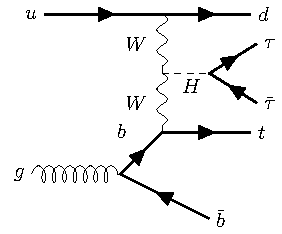
\includegraphics[width=0.9\textwidth]{/cephfs/user/s6chkirf/feynman_diagrams/tHq_tautau}\\
      \begin{itemize}
        \item n-jets: 2-6 (b-jets: \textbf{1})
        \item b-jet WP: 70 DL1r
        \item nLeptons \& nTaus: $\bf{1e / \mu~2\tau_{\text{had}}} $OS
        \item $E_{\text{T,miss}}$: no cut (to \SI{800}{GeV})
      \end{itemize}
    \end{column}
    \begin{column}{0.7\textwidth}
      \vspace*{-0.05\textwidth}
      \begin{itemize}
        \footnotesize
        \item jets:
        \vspace*{-0.02\textwidth}
        \begin{itemize}
          \footnotesize
          \item $p_T>\SI{25}{GeV}$
          \item $|\eta|<4.5$
          \item EMPFlow
        \end{itemize}
        \item electrons:
        \vspace*{-0.02\textwidth}
        \begin{itemize}
          \footnotesize
          \item $p_T>\SI{20}{GeV}$ trigger matched \SI{27}{GeV}
          \item $|\eta|<2.5$ not in 1.37 - 1.52
          \item WP: Tight ; \\isolation: PLIVTight
        \end{itemize}
        \item muons:
        \vspace*{-0.02\textwidth}
        \begin{itemize}
          \footnotesize
          \item $p_T>\SI{20}{GeV}$ trigger matched \SI{27}{GeV}
          \item $|\eta|<2.5$
          \item WP: Tight ; isolation: PLIVTight
        \end{itemize}
        \item taus:
        \vspace*{-0.02\textwidth}
        \begin{itemize}
          \footnotesize
          \item $p_T>\SI{20}{GeV}$ trigger matched \SI{27}{GeV}
          \item $|\eta|<2.5$ not in 1.37 - 1.52
          \item WP: RNNMedium
          \item ASG recommended OLR ($\tau_{had}$ remove jets)
        \end{itemize}
      \end{itemize}
    \end{column}
  \end{columns}
\end{frame}

\begin{frame}{Selection dileptau}
  \begin{columns}
    \begin{column}{0.5\textwidth}
      \centering 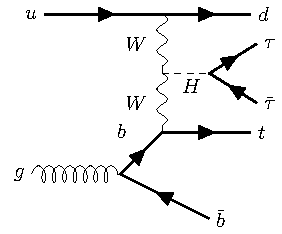
\includegraphics[width=0.9\textwidth]{/cephfs/user/s6chkirf/feynman_diagrams/tHq_tautau}\\
      \begin{itemize}
        \item n-jets: 2-6 (b-jets: \textbf{1})
        \item b-jet WP: 70 DL1r
        \item nLeptons \& nTaus: $\bf{2e / \mu~1\tau_{\text{had}}} $(1 OS light lepton)
        \item $E_{\text{T,miss}}$: no cut (to \SI{800}{GeV})
      \end{itemize}
    \end{column}
    \begin{column}{0.7\textwidth}
      \vspace*{-0.05\textwidth}
      \begin{itemize}
        \footnotesize
        \item jets:
        \vspace*{-0.02\textwidth}
        \begin{itemize}
          \footnotesize
          \item $p_T>\SI{25}{GeV}$
          \item $|\eta|<4.5$
          \item EMPFlow
        \end{itemize}
        \item electrons:
        \vspace*{-0.02\textwidth}
        \begin{itemize}
          \footnotesize
          \item $p_T>\SI{20}{GeV}$ trigger matched \SI{27}{GeV}
          \item $|\eta|<2.5$ not in 1.37 - 1.52
          \item WP: Tight ; \\isolation: PLIVTight
        \end{itemize}
        \item muons:
        \vspace*{-0.02\textwidth}
        \begin{itemize}
          \footnotesize
          \item $p_T>\SI{20}{GeV}$ trigger matched \SI{27}{GeV}
          \item $|\eta|<2.5$
          \item WP: Tight ; isolation: PLIVTight
        \end{itemize}
        \item taus:
        \vspace*{-0.02\textwidth}
        \begin{itemize}
          \footnotesize
          \item $p_T>\SI{20}{GeV}$ trigger matched \SI{27}{GeV}
          \item $|\eta|<2.5$ not in 1.37 - 1.52
          \item WP: RNNMedium
          \item ASG recommended OLR ($\tau_{had}$ remove jets)
        \end{itemize}
      \end{itemize}
    \end{column}
  \end{columns}
\end{frame}
\section*{Region definitions}
\begin{frame}{Region definitions dileptau}
    \begin{columns}
        \begin{column}{0.6\textwidth}
            \begin{figure}
                \centering
                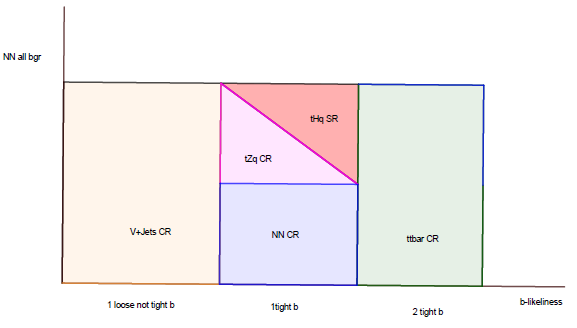
\includegraphics[width=\textwidth]{region_defs}
            \end{figure}
        \end{column}
        \begin{column}{0.4\textwidth}
            \begin{enumerate}
                \item Cut on number ob b-jets
                \item Cut on MVA score
                \item Separate \tZq
            \end{enumerate}
        \end{column}
    \end{columns}
    \begin{figure}
        \centering
        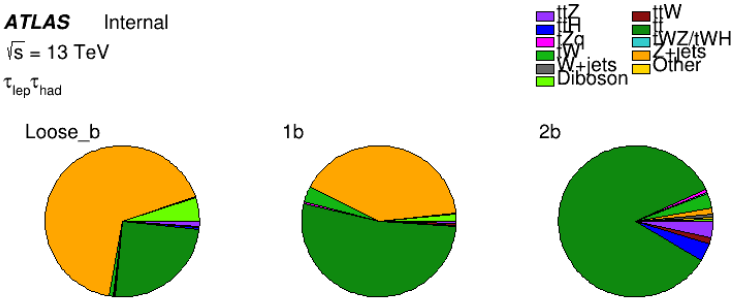
\includegraphics[width=0.76\textwidth]{lephad_yield}
    \end{figure}
\end{frame}

\begin{frame}{Region definitions lepditau}
    \begin{columns}
        \begin{column}{0.6\textwidth}
            \begin{figure}
                \centering
                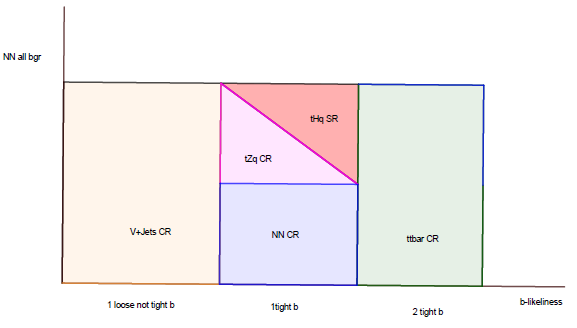
\includegraphics[width=0.8\textwidth]{region_defs}
            \end{figure}
        \end{column}
        \begin{column}{0.4\textwidth}
            \begin{enumerate}
                \item Cut on number ob b-jets
                \item Cut on MVA score
                \item Separate \tZq
            \end{enumerate}
        \end{column}
    \end{columns}
    \begin{figure}
        \centering
        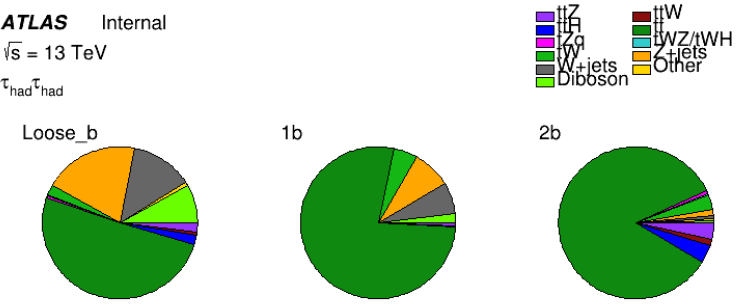
\includegraphics[width=0.76\textwidth]{hadhad_yield}
    \end{figure}
\end{frame}
\section*{MVA}
\begin{frame}{Lepditau Neural network}
    \begin{columns}
        \begin{column}{0.5\textwidth}
            \begin{figure}
                \centering
                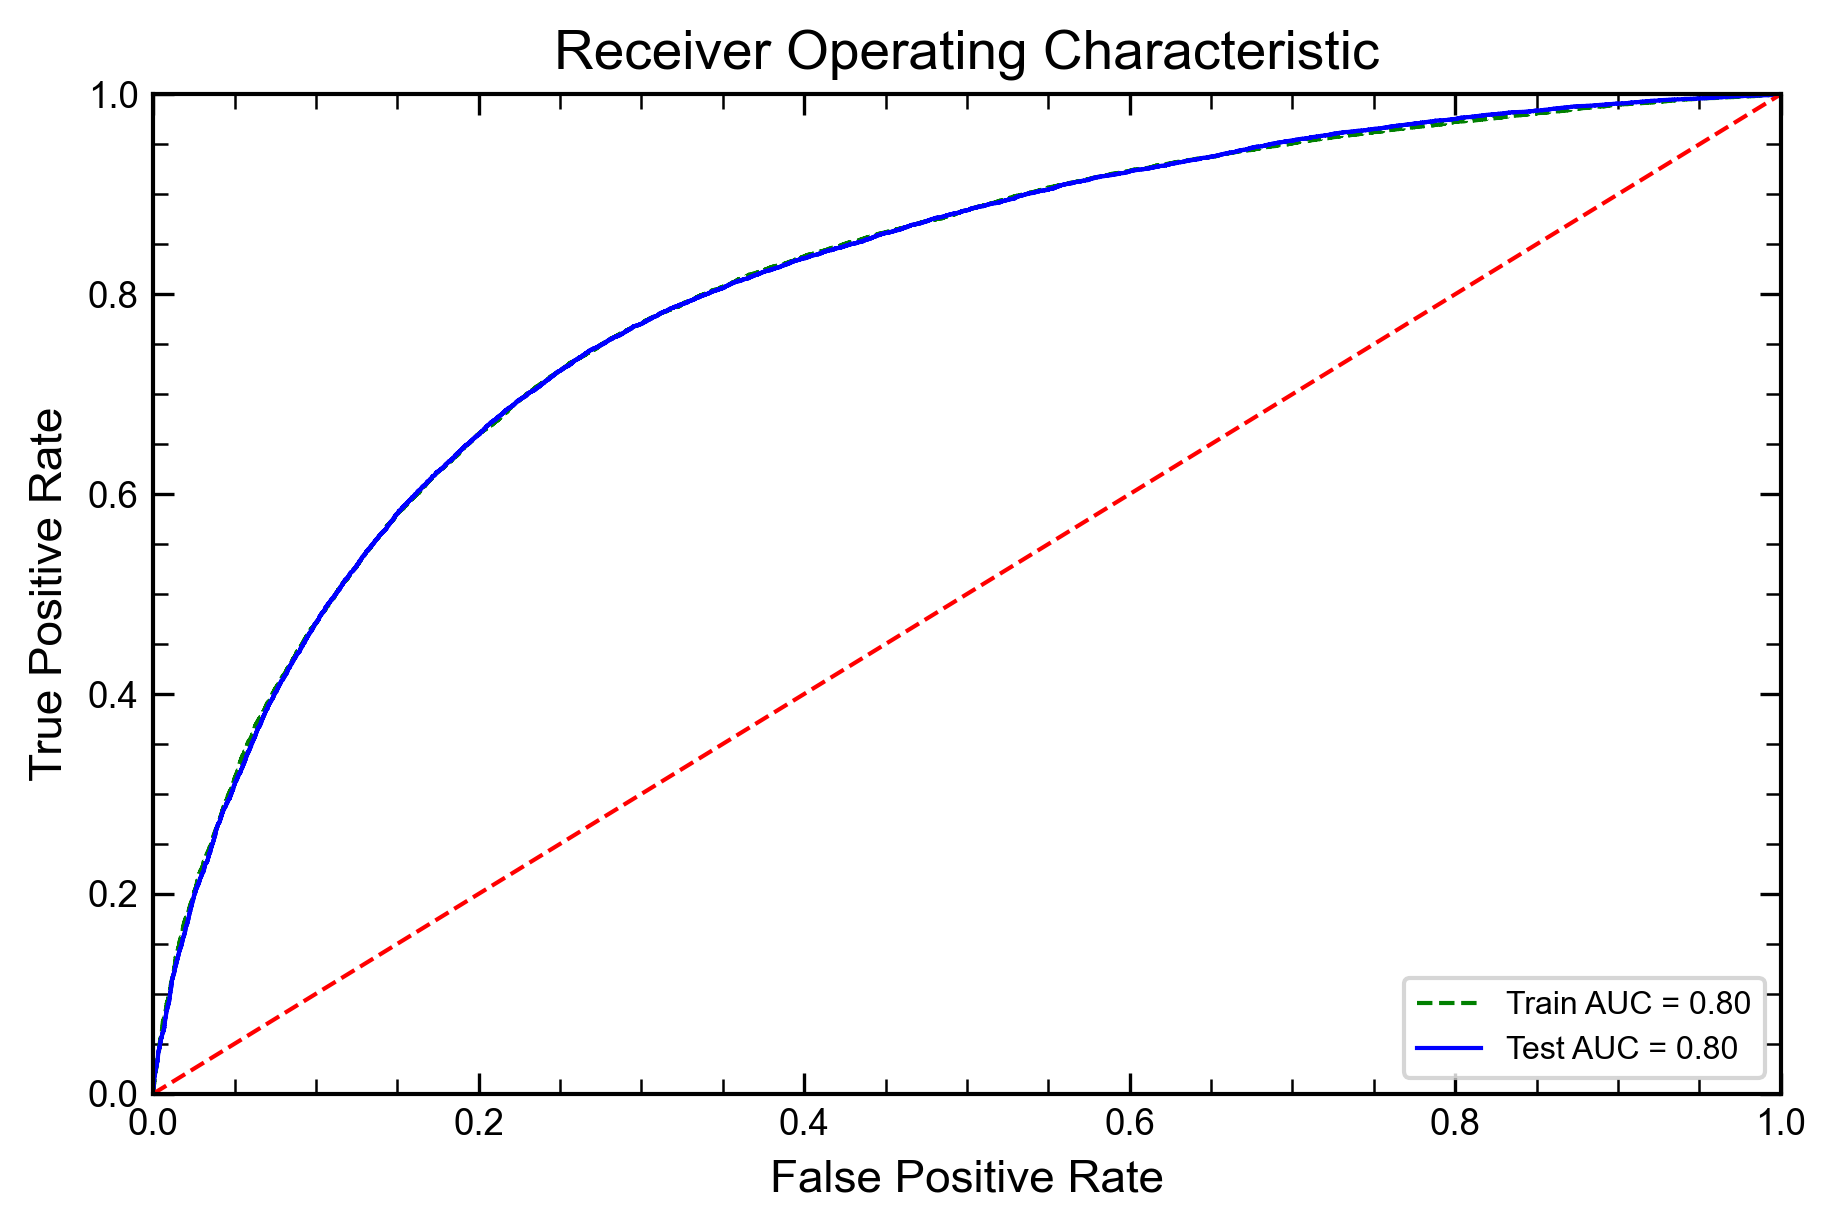
\includegraphics[width=0.8\textwidth]{hadhad_ROC}    
            \end{figure}
            \vspace{-0.35cm}
            \begin{figure}
                \centering
                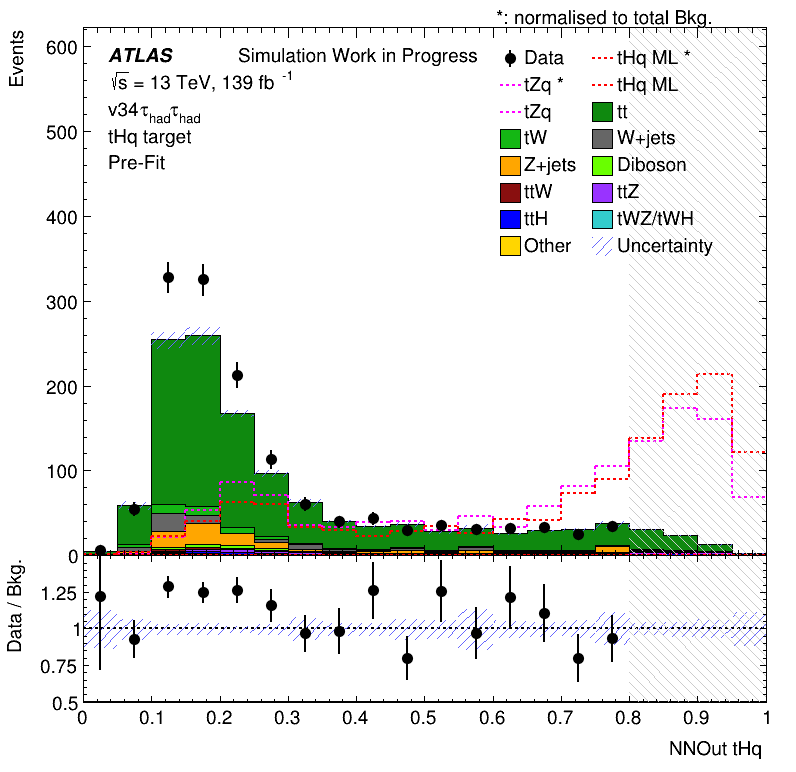
\includegraphics[width=0.8\textwidth]{NNOut_hadhad}    
            \end{figure}
        \end{column}
        \begin{column}{0.5\textwidth}
            \vspace{-0.25cm}
            \begin{block}{Setup}
                \begin{itemize}
                    \item Optimisation: Evolutionary + grid search
                    \item Model: Categorical (currently binary for v34)
                    \item Variables: final state kinematics
                    \item Currently performance problems for v34
                    \item Train on absolute, predict on full weights
                \end{itemize}
            \end{block}
            \vspace{-0.45cm}
            \begin{block}{Plans}
                \begin{itemize}
                    \item Validate categorical setup in lepditau
                    \item Rerun the optimisation for v34
                    \item Rank and test variables
                \end{itemize} 
             \end{block}
        \end{column}
    \end{columns}
\end{frame}

\begin{frame}{Dileptau Neural network}
    \begin{columns}
        \begin{column}{0.5\textwidth}
            \begin{figure}
                \centering
                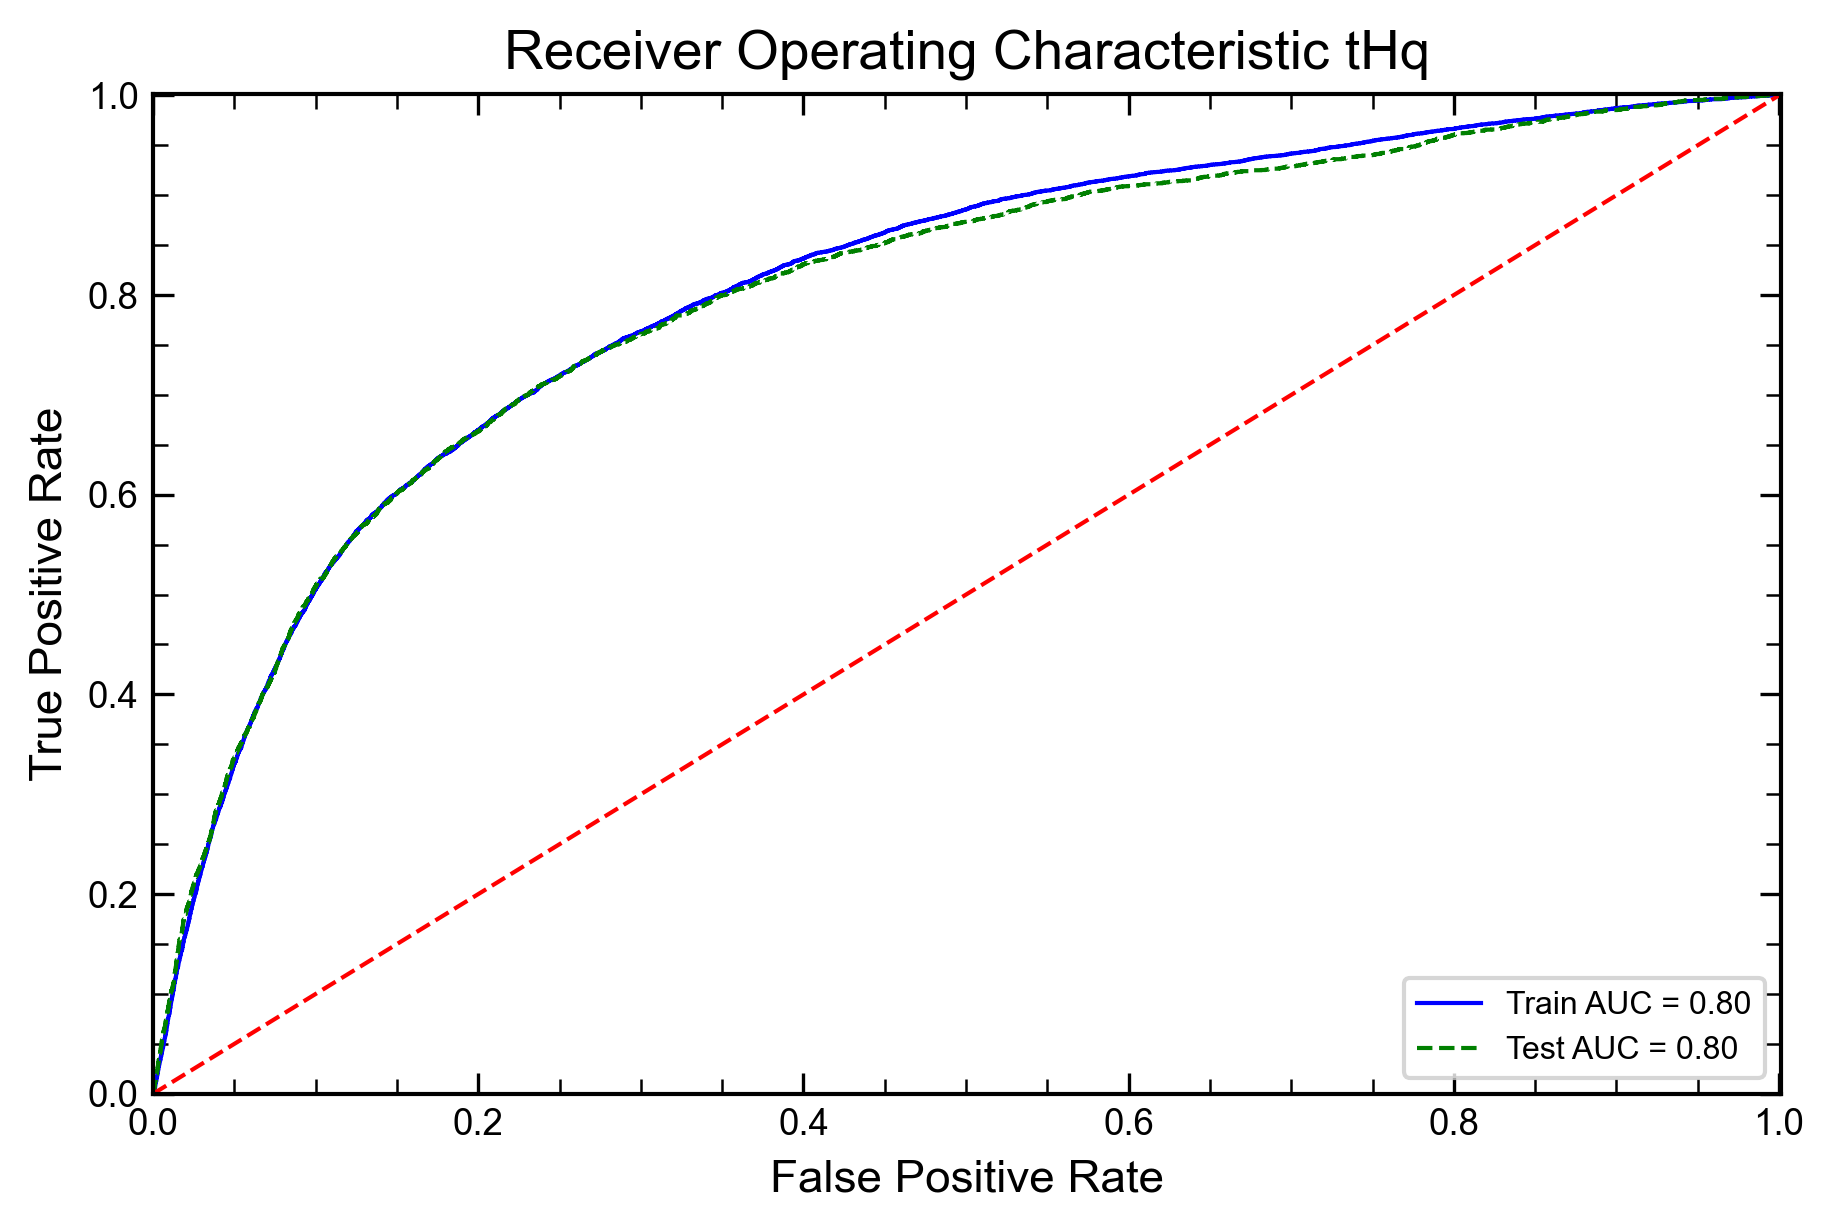
\includegraphics[width=0.8\textwidth]{lephad_ROC}    
            \end{figure}
            \vspace{-0.35cm}
            \begin{figure}
                \centering
                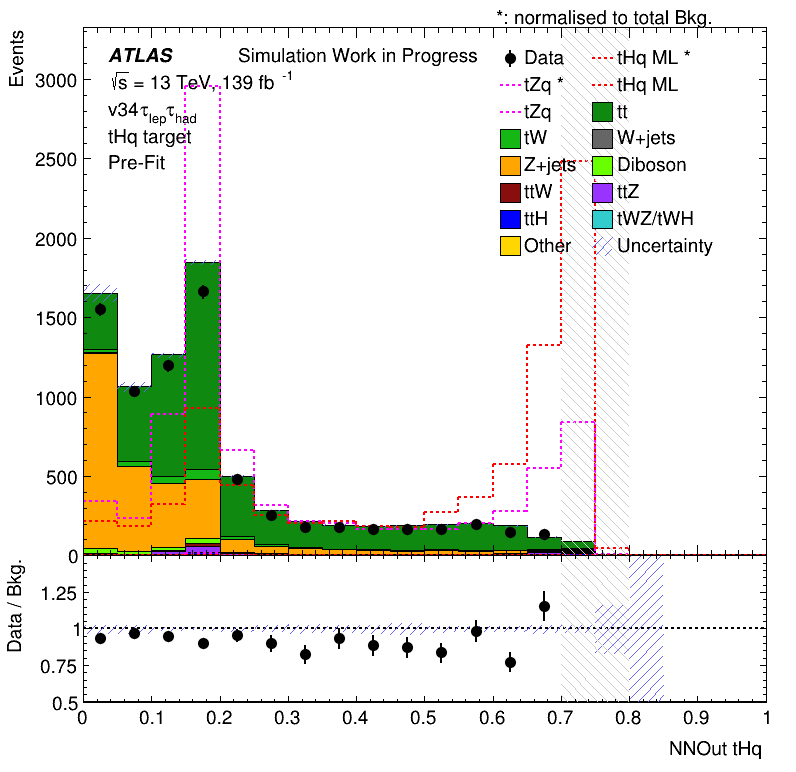
\includegraphics[width=0.8\textwidth]{lephad_2}    
            \end{figure}
        \end{column}
        \begin{column}{0.5\textwidth}
            \begin{block}{Setup}
                \begin{itemize}
                    \item Optimisation: Evolutionary + grid search
                    \item Model: Categorical (Treating \tZq separately)
                    \item Variables: final state kinematics
                    \item Train on absolute, predict on full weights
                \end{itemize}
            \end{block}
            \vspace{-0.2cm}
            \begin{block}{Plans}
               \begin{itemize}
                   \item Rerun the optimisation for v34
                   \item Rank and test variables
               \end{itemize} 
            \end{block}
        \end{column}
    \end{columns}
\end{frame}

\begin{frame}{Dileptau S/B}
    \begin{columns}
        \begin{column}{0.5\textwidth}
            \begin{figure}
                \centering
                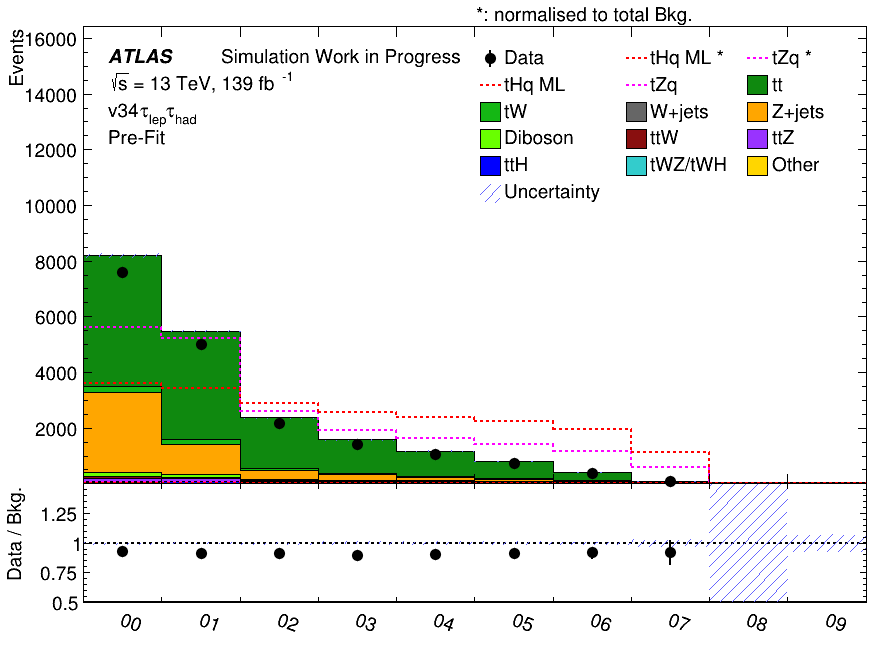
\includegraphics[width=\textwidth]{lephad_cutflow}
            \end{figure}
        \end{column}
        \begin{column}{0.5\textwidth}
            \begin{figure}
                \centering
                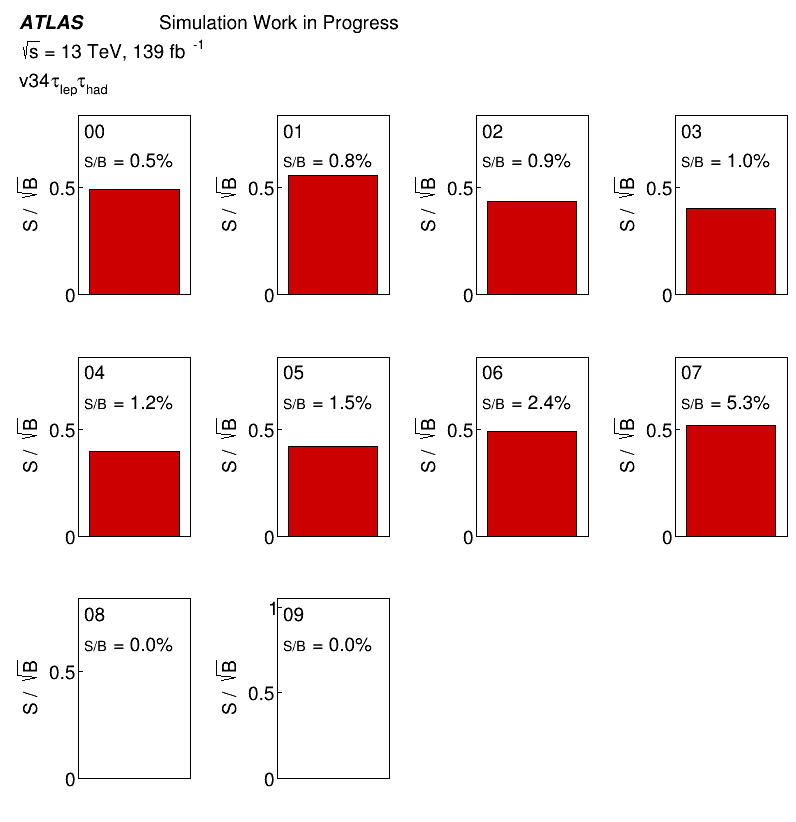
\includegraphics[width=\textwidth]{NN_sb}
            \end{figure}
        \end{column}
    \end{columns}
\end{frame}

\begin{frame}{Dileptau BDT}
    \begin{figure}
        \centering
        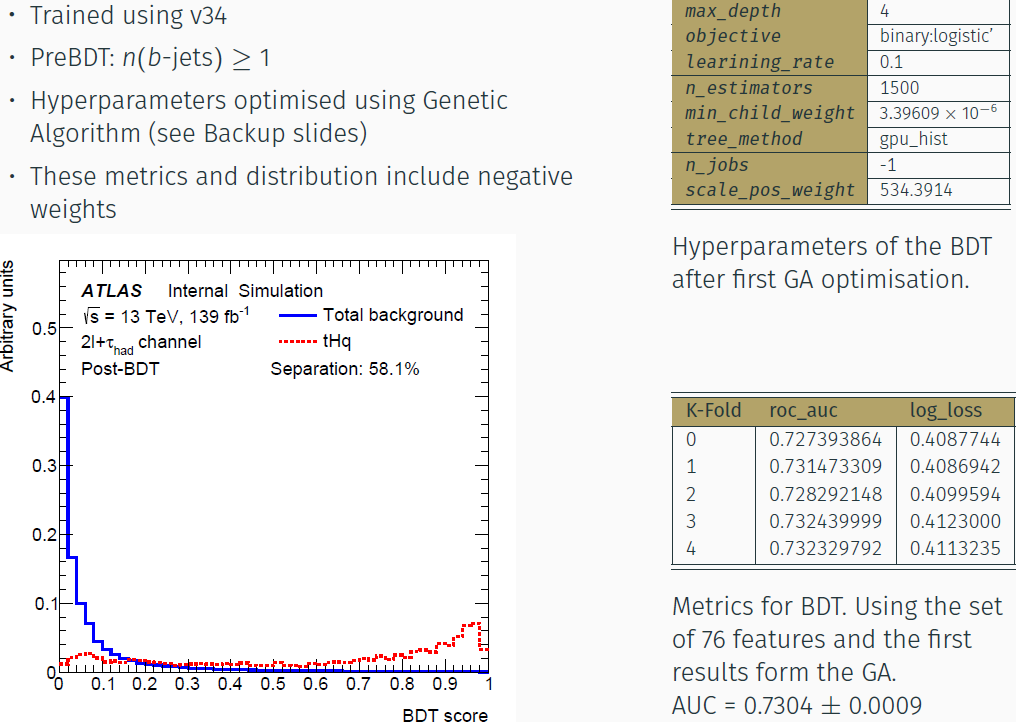
\includegraphics[width=0.9\textwidth]{BDT1}
    \end{figure}
\end{frame}

\begin{frame}{Dileptau BDT}
    \begin{figure}
        \centering
        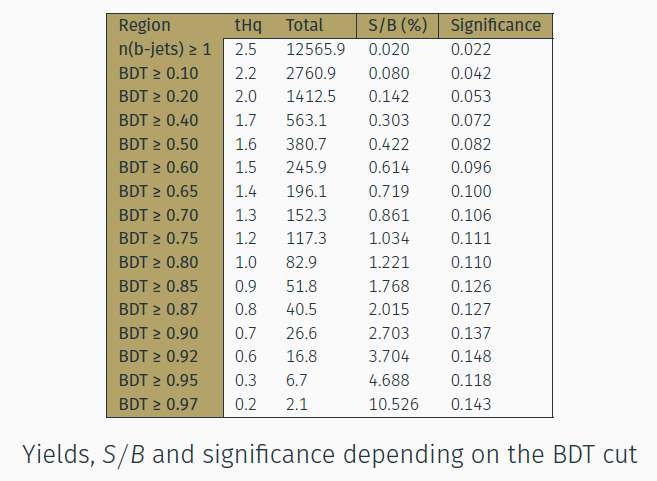
\includegraphics[width=0.9\textwidth]{BDT2}
    \end{figure}
\end{frame}

\begin{frame}{Dileptau BDT}
    \begin{itemize}
        \item BDT not using categorical approach
        \item \tZq separation is still quite good
    \end{itemize}
    \begin{figure}
        \centering
        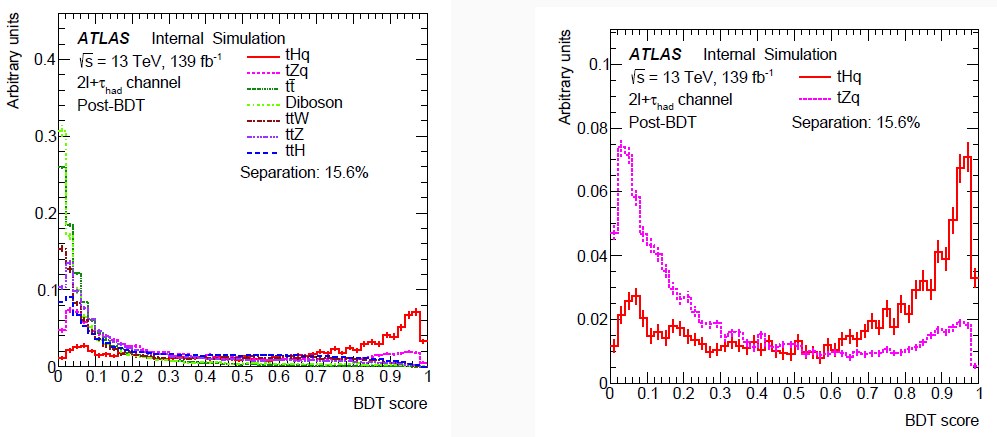
\includegraphics[width=0.9\textwidth]{BDT3}
    \end{figure}
\end{frame}

\section*{Methods}
\begin{frame}{Fake estimation dileptau}
    \begin{figure}
        \centering
        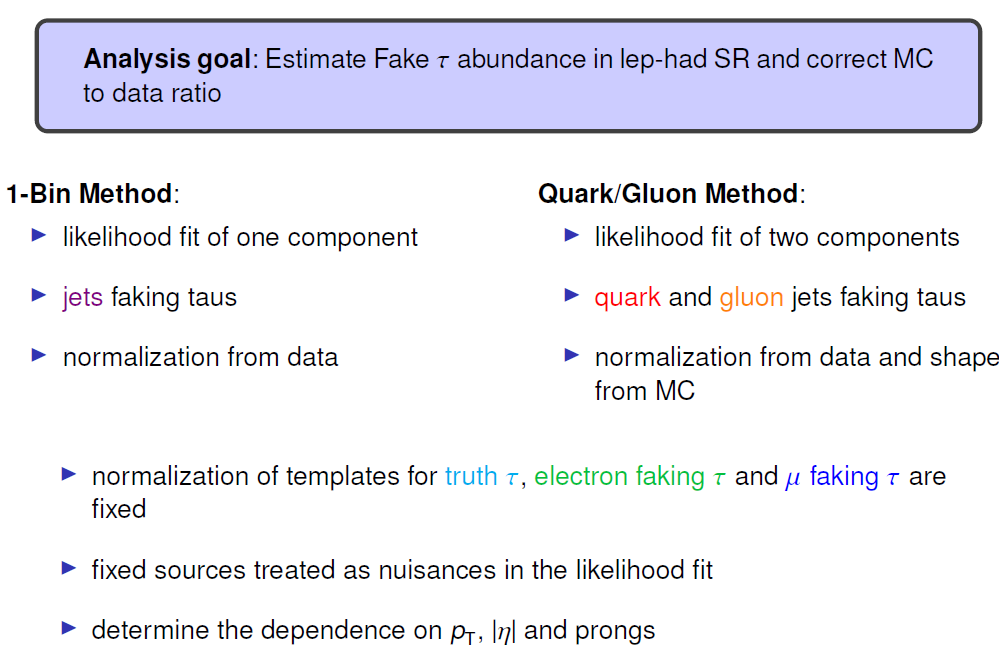
\includegraphics[width=\textwidth]{fake_strategy}
    \end{figure}
\end{frame}
 
\begin{frame}{One bin method dileptau Control Region}
    \begin{figure}
        \centering
        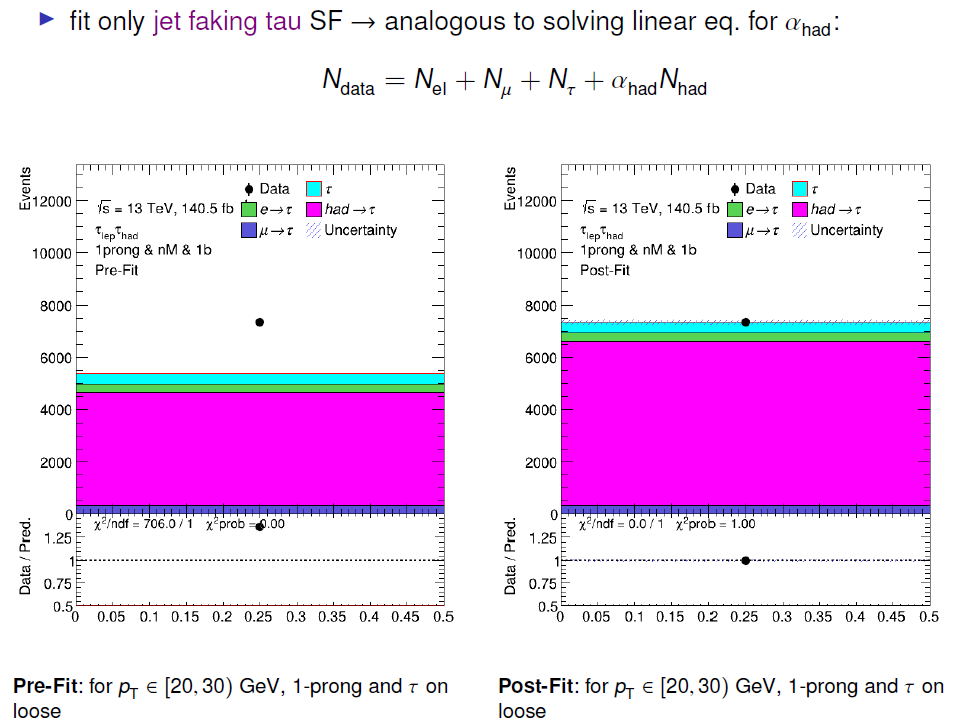
\includegraphics[width=0.85\textwidth]{oneBinCR}
    \end{figure}
\end{frame}

\begin{frame}{One bin method dileptau Signal Region}
    \begin{figure}
        \centering
        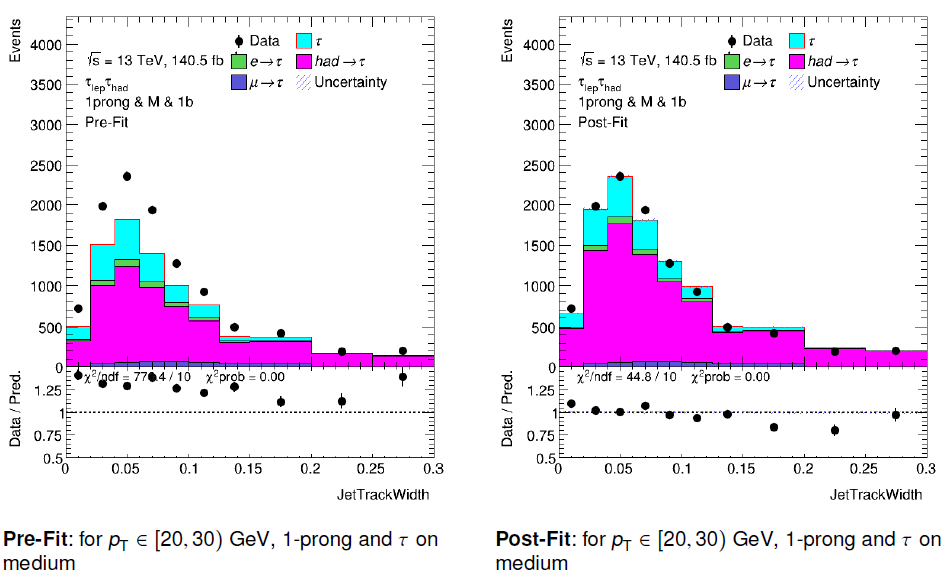
\includegraphics[width=0.85\textwidth]{oneBinSR}
    \end{figure}
\end{frame}

\begin{frame}{Quark/gluon method dileptau Control Region}
    \begin{figure}
        \centering
        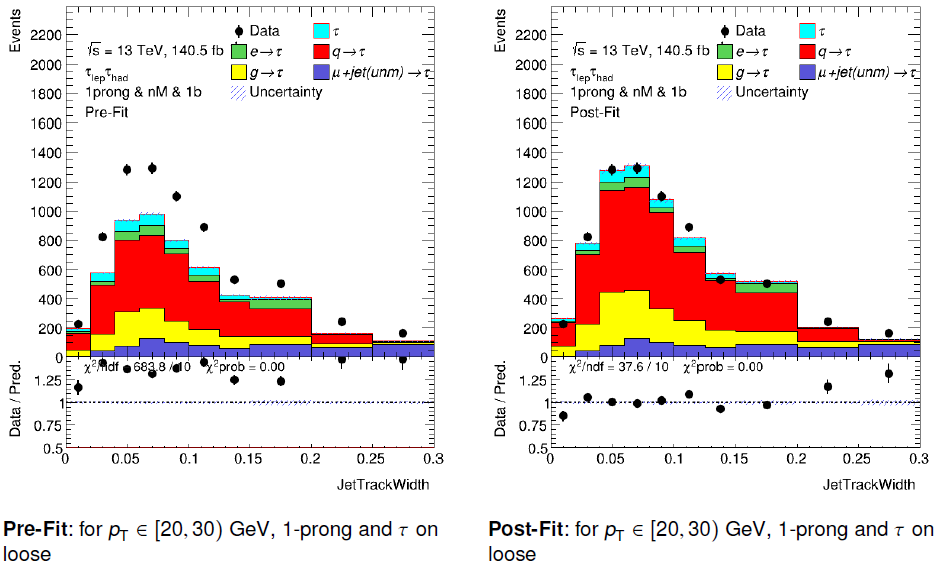
\includegraphics[width=0.95\textwidth]{quarkGluonCR}
    \end{figure}
\end{frame}

\begin{frame}{Quark/gluon method dileptau Signal Region}
    \begin{figure}
        \centering
        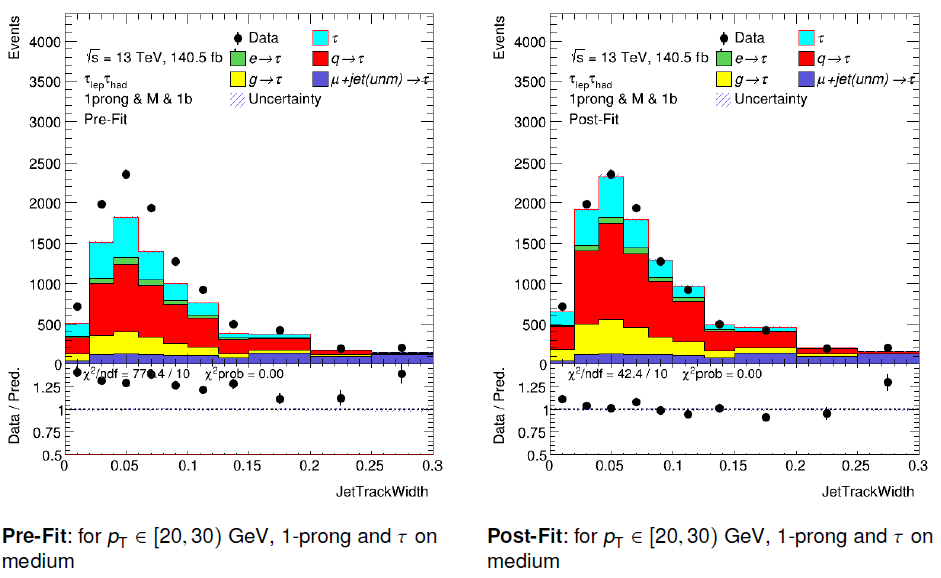
\includegraphics[width=0.95\textwidth]{quarkGluonSR}
    \end{figure}
\end{frame}

\begin{frame}{Fake Estimation Lepditau}
    \begin{itemize}
        \item Using template fit method
    \end{itemize}
    \begin{columns}
        \begin{column}{0.5\textwidth}
            \begin{figure}
                \centering
                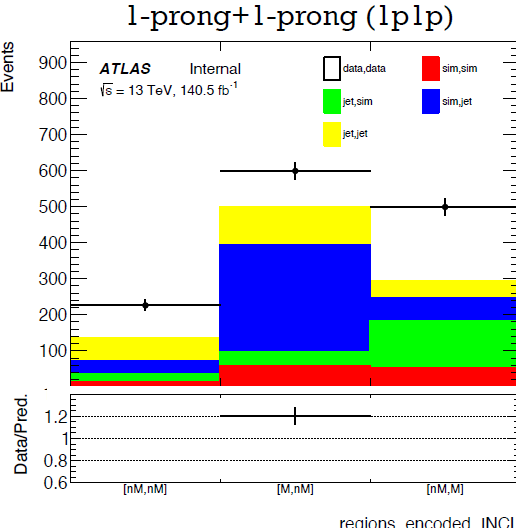
\includegraphics[width=\textwidth]{oleh_1}
            \end{figure}
        \end{column}
        \begin{column}{0.5\textwidth}
            \begin{figure}
                \centering
                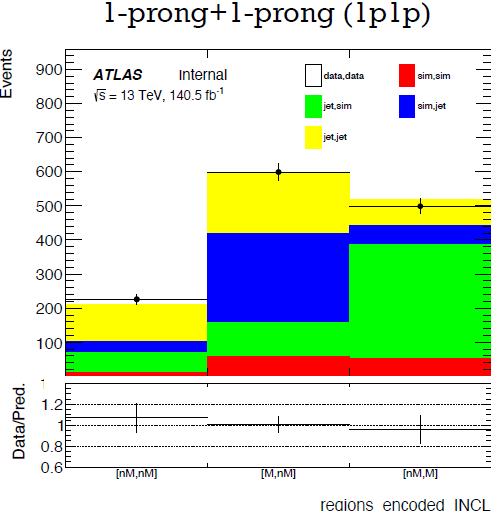
\includegraphics[width=\textwidth]{oleh_2}
            \end{figure}
        \end{column}
    \end{columns}
\end{frame}

\begin{frame}{Lepditau fake estimation fit results}
    \begin{figure}
        \centering
        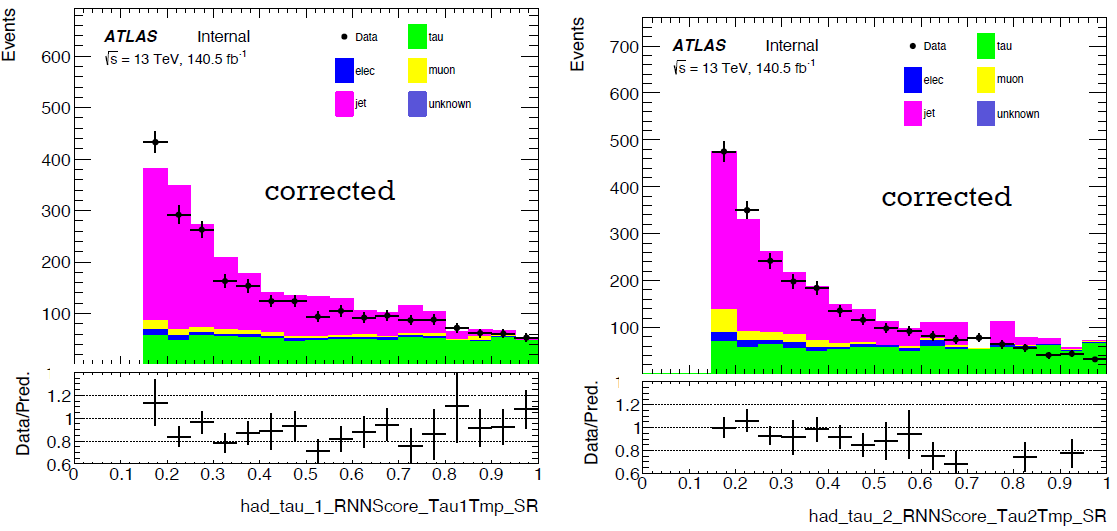
\includegraphics[width=\textwidth]{oleh_3}
    \end{figure}
\end{frame}

\begin{frame}{Lepditau fake estimation fit results}
    \begin{figure}
        \centering
        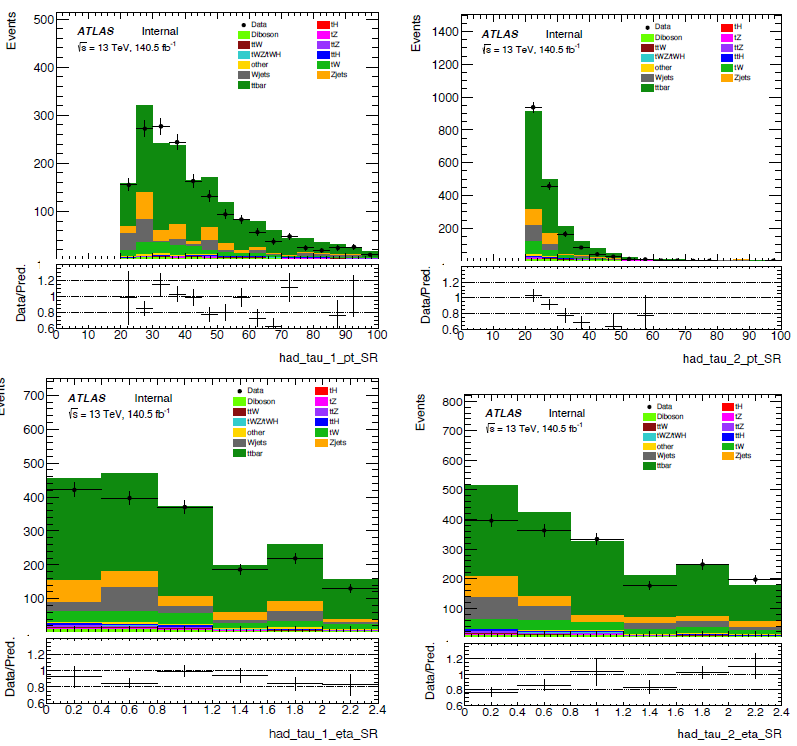
\includegraphics[width=0.74\textwidth]{oleh_4}
    \end{figure}
\end{frame}

\begin{frame}{Lepton Assigment Method}
    \begin{itemize}
        \item Establish method for lepton assignment
        \vspace{0.6cm}
        \item Tested promising variables for assignment
        \vspace{0.6cm}
        \item $m_{pred,t}(lep(Higgs)) - m_{pred,t}(lep(top)) > 0$
        \vspace{0.6cm}
        \item Generality allows to expand to SS events
    \end{itemize}
\end{frame}

\begin{frame}{Lepton Assigment Results}
    \begin{figure}
        \centering
        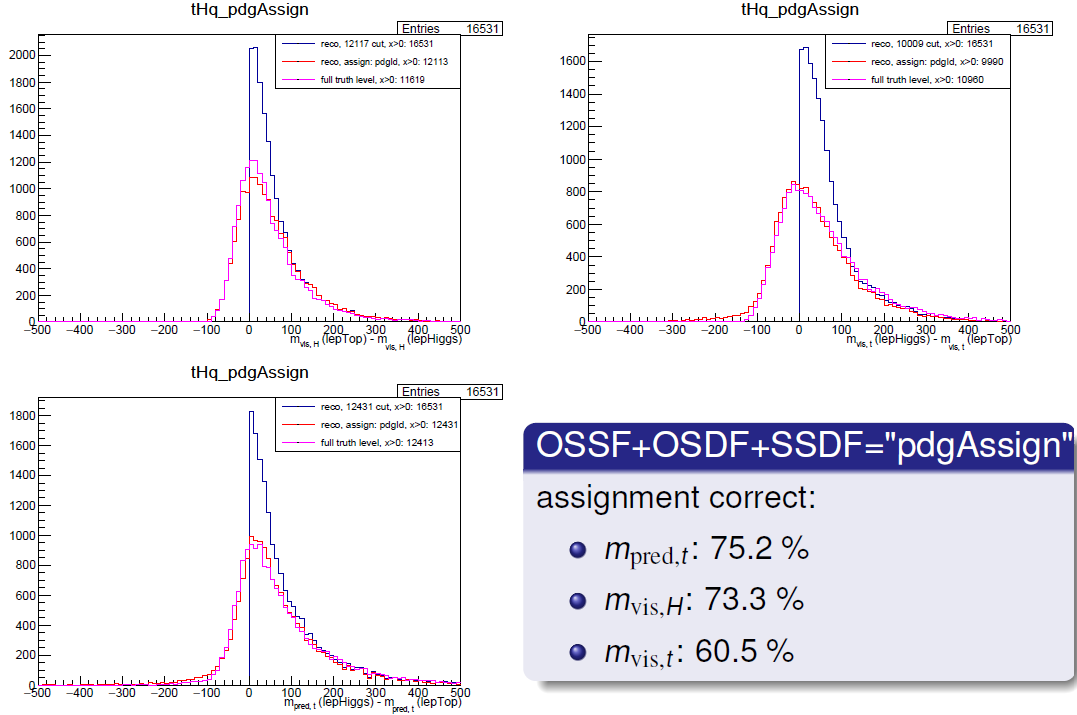
\includegraphics[width=0.9\textwidth]{assignment_results}
    \end{figure}
\end{frame}

\section*{Fit model}
\begin{frame}{First fit results dileptau}
    \begin{columns}
        \begin{column}{0.5\textwidth}
            \begin{figure}
                \centering
                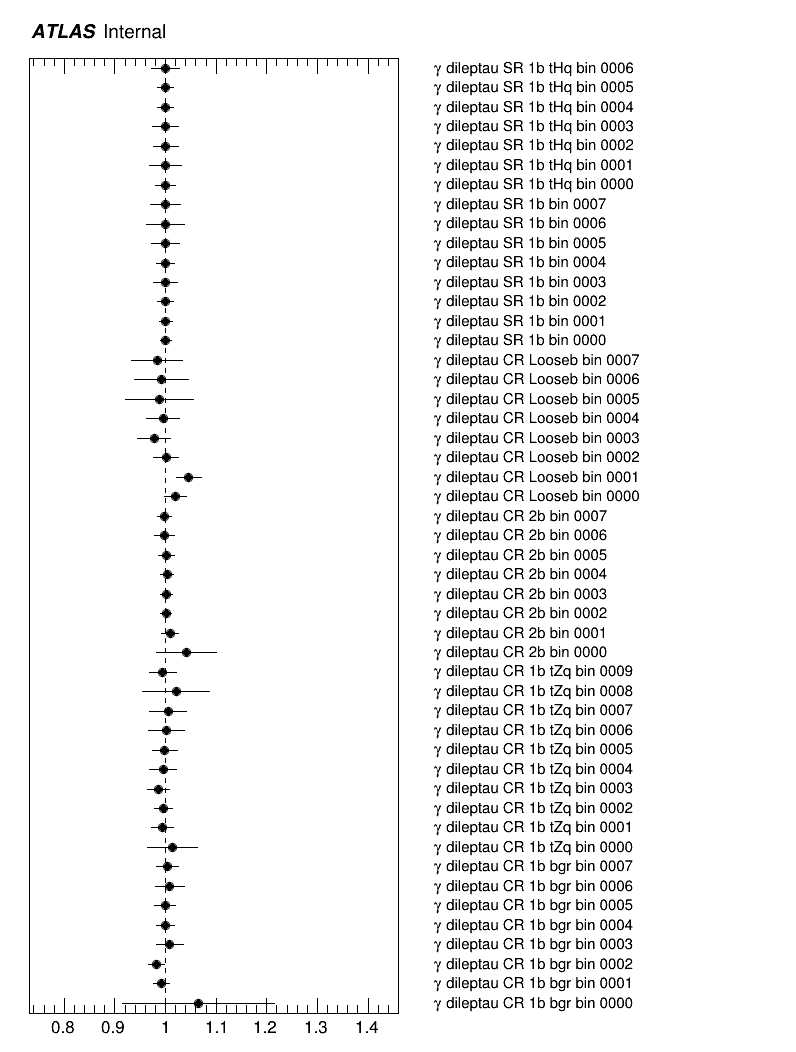
\includegraphics[width=\textwidth]{asimov}
            \end{figure}
        \end{column}
        \begin{column}{0.5\textwidth}
            \begin{figure}
                \centering
                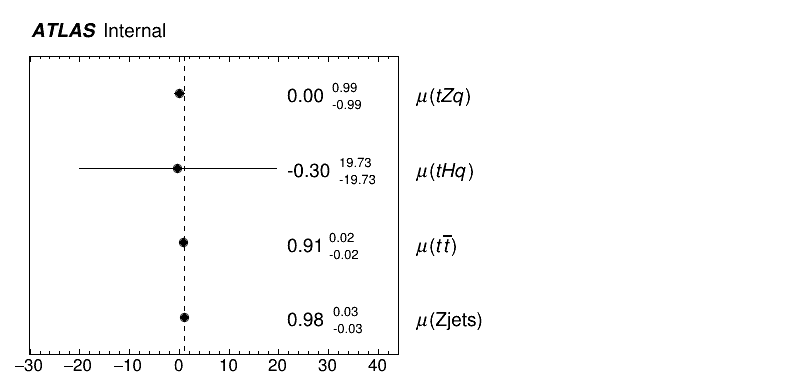
\includegraphics[width=\textwidth]{fit}
            \end{figure}
            \begin{itemize}
                \item Technically fitting is possible
                \item Much room for improvement left
                \item Separation for V+jets and \ttbar already good
                \item Higher sensitivity expected from SS event inclusion
            \end{itemize}
        \end{column}
    \end{columns}
\end{frame}

\begin{frame}{First fit results dileptau}
    \begin{columns}
        \begin{column}{0.5\textwidth}
            \begin{figure}
                \centering
                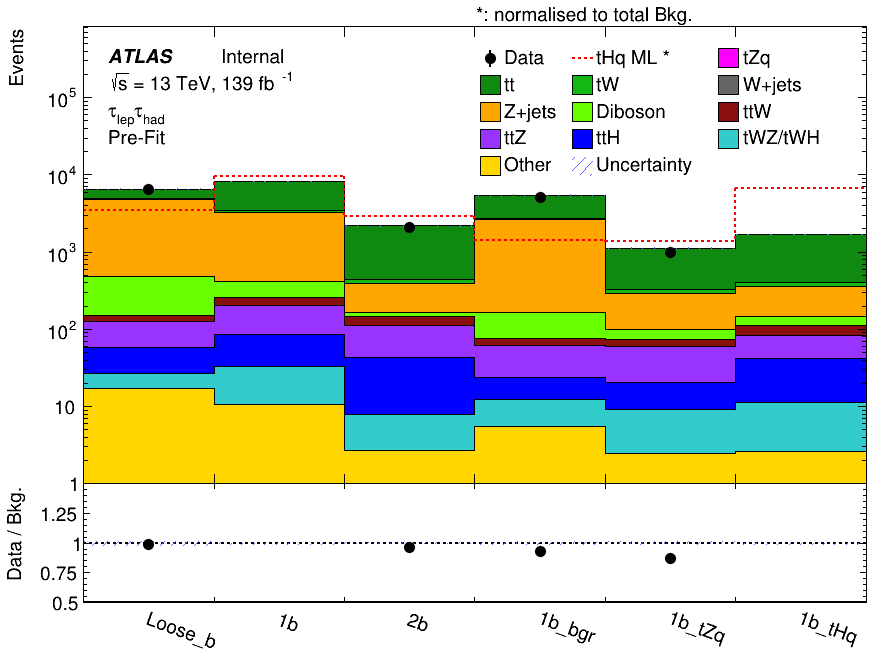
\includegraphics[width=\textwidth]{prefot}
            \end{figure}
        \end{column}
        \begin{column}{0.5\textwidth}
            \begin{figure}
                \centering
                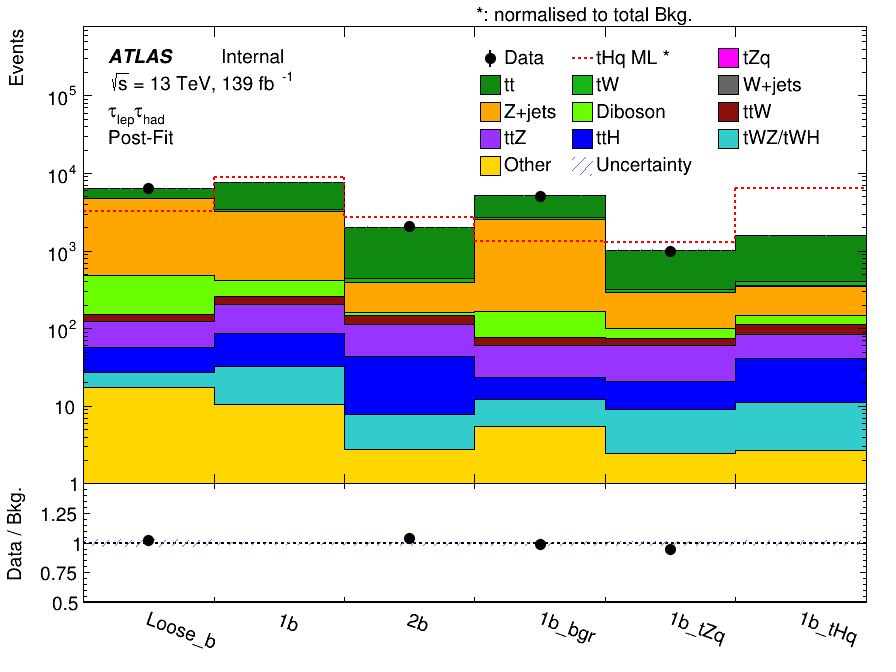
\includegraphics[width=\textwidth]{postfit}
            \end{figure}
        \end{column}
    \end{columns}
\end{frame}

\begin{frame}{First fit results lepditau}
    \begin{columns}
        \begin{column}{0.5\textwidth}
            \begin{figure}
                \centering
                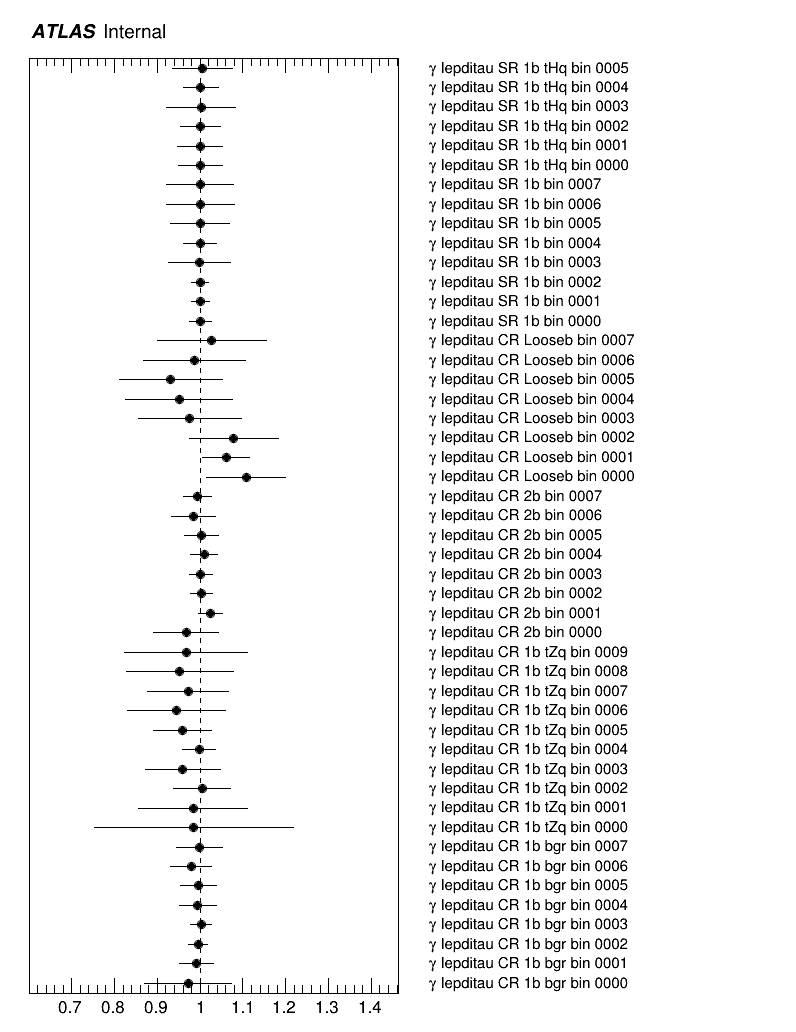
\includegraphics[width=\textwidth]{asimov_hadhad}
            \end{figure}
        \end{column}
        \begin{column}{0.5\textwidth}
            \begin{figure}
                \centering
                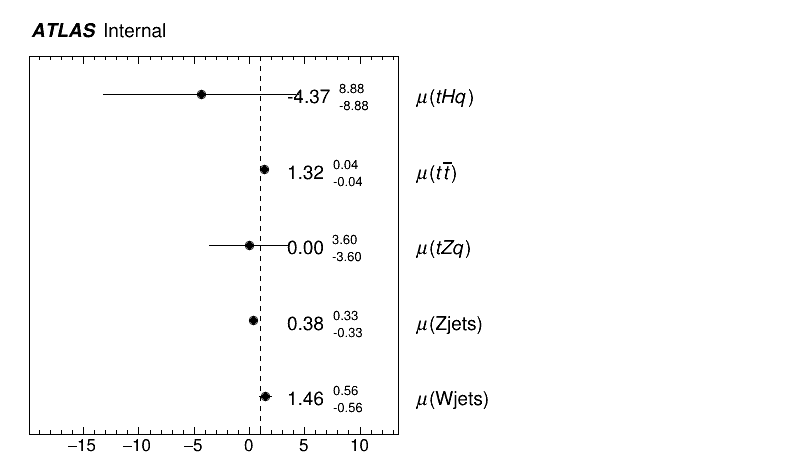
\includegraphics[width=\textwidth]{fit_hadhad}
            \end{figure}
            \begin{itemize}
                \item Technically fitting is possible
                \item Much room for improvement left
                \item Separation for V+jets and \ttbar already good
                \item Improvement in fake tau scale factors to be expected
            \end{itemize}
        \end{column}
    \end{columns}
\end{frame}

\begin{frame}{First fit results lepditau}
    \begin{columns}
        \begin{column}{0.5\textwidth}
            \begin{figure}
                \centering
                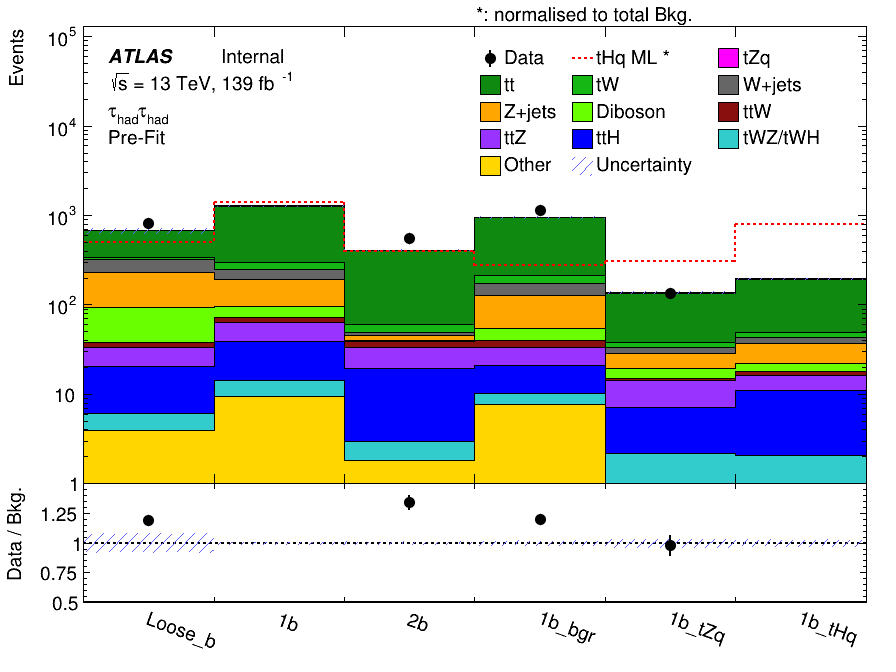
\includegraphics[width=\textwidth]{prefit_hadhad}
            \end{figure}
        \end{column}
        \begin{column}{0.5\textwidth}
            \begin{figure}
                \centering
                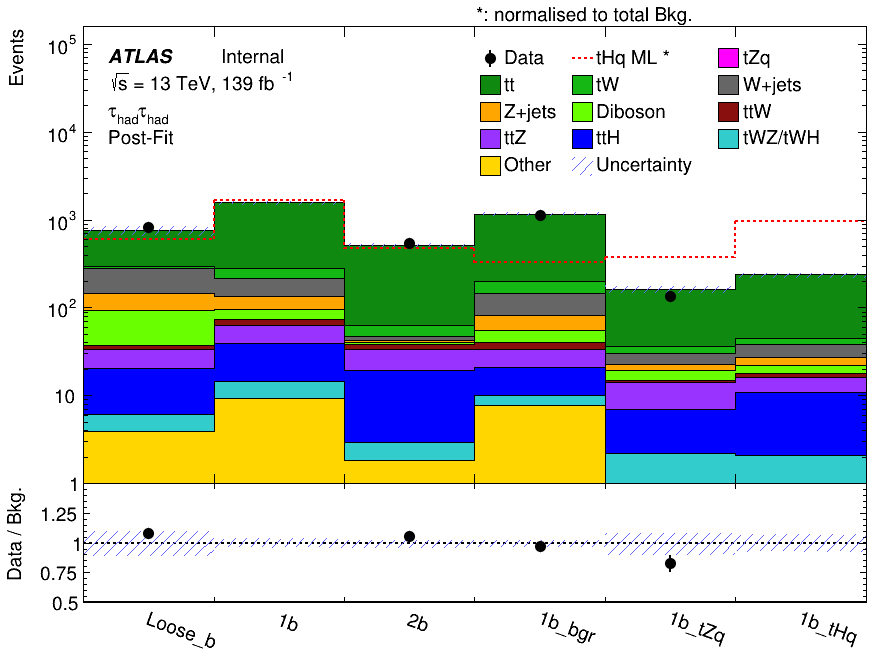
\includegraphics[width=\textwidth]{postfit_hadhad}
            \end{figure}
        \end{column}
    \end{columns}
\end{frame}
\section*{Int note}
\begin{frame}{Status of the Int Note}
    \begin{itemize}
        \item \url{https://gitlab.cern.ch/atlas-physics-office/HIGG/ANA-HIGG-2020-02/ANA-HIGG-2020-02-INT1}
        \item Majority is finished
        \item For all the missing parts authors have been assigned and have accepted
        \item A first version is planned for next week
    \end{itemize}
\end{frame}

\begin{frame}{More information}
    \begin{itemize}
        \item \href{https://indico.cern.ch/event/1073925/contributions/4516262/attachments/2338336/3986788/14-10-21_overview.pdf}{Checks on v34}
        \item \href{https://indico.cern.ch/event/1073925/contributions/4516262/attachments/2338336/3993194/TauFakes_lep2tau.pdf}{Lepditau Fakes}        
        \item \href{https://indico.cern.ch/event/1073925/contributions/4516262/attachments/2338336/3986886/dileptau_fakes.pdf}{Dileptau Fakes}
        \item \href{https://indico.cern.ch/event/1073925/contributions/4516262/attachments/2338336/3993953/categorical_MVA.pdf}{Categorical MVA}
        \item Dileptau \href{https://indico.cern.ch/event/1073925/contributions/4516262/attachments/2340922/3993860/tHq_2L1Tau_v34_BDTstatus.pdf}{BDT}, \href{https://indico.cern.ch/event/1073925/contributions/4516262/attachments/2340922/3993071/FeatureOptimise.pdf}{feature importance} 
        \item \href{https://indico.cern.ch/event/1073925/contributions/4516262/attachments/2338336/3990127/LeptonAssignment_Reco_3.pdf}{Lepton assignment}
    \end{itemize}
\end{frame}









\end{document}